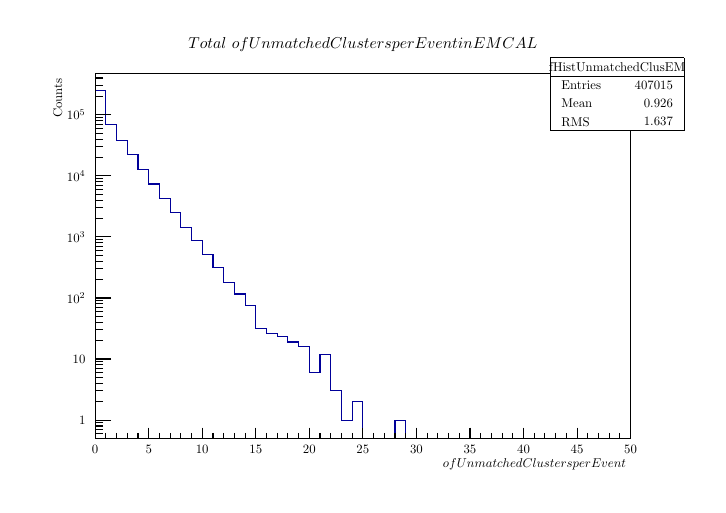
\begin{tikzpicture}
\pgfdeclareplotmark{cross} {
\pgfpathmoveto{\pgfpoint{-0.3\pgfplotmarksize}{\pgfplotmarksize}}
\pgfpathlineto{\pgfpoint{+0.3\pgfplotmarksize}{\pgfplotmarksize}}
\pgfpathlineto{\pgfpoint{+0.3\pgfplotmarksize}{0.3\pgfplotmarksize}}
\pgfpathlineto{\pgfpoint{+1\pgfplotmarksize}{0.3\pgfplotmarksize}}
\pgfpathlineto{\pgfpoint{+1\pgfplotmarksize}{-0.3\pgfplotmarksize}}
\pgfpathlineto{\pgfpoint{+0.3\pgfplotmarksize}{-0.3\pgfplotmarksize}}
\pgfpathlineto{\pgfpoint{+0.3\pgfplotmarksize}{-1.\pgfplotmarksize}}
\pgfpathlineto{\pgfpoint{-0.3\pgfplotmarksize}{-1.\pgfplotmarksize}}
\pgfpathlineto{\pgfpoint{-0.3\pgfplotmarksize}{-0.3\pgfplotmarksize}}
\pgfpathlineto{\pgfpoint{-1.\pgfplotmarksize}{-0.3\pgfplotmarksize}}
\pgfpathlineto{\pgfpoint{-1.\pgfplotmarksize}{0.3\pgfplotmarksize}}
\pgfpathlineto{\pgfpoint{-0.3\pgfplotmarksize}{0.3\pgfplotmarksize}}
\pgfpathclose
\pgfusepathqstroke
}
\pgfdeclareplotmark{cross*} {
\pgfpathmoveto{\pgfpoint{-0.3\pgfplotmarksize}{\pgfplotmarksize}}
\pgfpathlineto{\pgfpoint{+0.3\pgfplotmarksize}{\pgfplotmarksize}}
\pgfpathlineto{\pgfpoint{+0.3\pgfplotmarksize}{0.3\pgfplotmarksize}}
\pgfpathlineto{\pgfpoint{+1\pgfplotmarksize}{0.3\pgfplotmarksize}}
\pgfpathlineto{\pgfpoint{+1\pgfplotmarksize}{-0.3\pgfplotmarksize}}
\pgfpathlineto{\pgfpoint{+0.3\pgfplotmarksize}{-0.3\pgfplotmarksize}}
\pgfpathlineto{\pgfpoint{+0.3\pgfplotmarksize}{-1.\pgfplotmarksize}}
\pgfpathlineto{\pgfpoint{-0.3\pgfplotmarksize}{-1.\pgfplotmarksize}}
\pgfpathlineto{\pgfpoint{-0.3\pgfplotmarksize}{-0.3\pgfplotmarksize}}
\pgfpathlineto{\pgfpoint{-1.\pgfplotmarksize}{-0.3\pgfplotmarksize}}
\pgfpathlineto{\pgfpoint{-1.\pgfplotmarksize}{0.3\pgfplotmarksize}}
\pgfpathlineto{\pgfpoint{-0.3\pgfplotmarksize}{0.3\pgfplotmarksize}}
\pgfpathclose
\pgfusepathqfillstroke
}
\pgfdeclareplotmark{newstar} {
\pgfpathmoveto{\pgfqpoint{0pt}{\pgfplotmarksize}}
\pgfpathlineto{\pgfqpointpolar{44}{0.5\pgfplotmarksize}}
\pgfpathlineto{\pgfqpointpolar{18}{\pgfplotmarksize}}
\pgfpathlineto{\pgfqpointpolar{-20}{0.5\pgfplotmarksize}}
\pgfpathlineto{\pgfqpointpolar{-54}{\pgfplotmarksize}}
\pgfpathlineto{\pgfqpointpolar{-90}{0.5\pgfplotmarksize}}
\pgfpathlineto{\pgfqpointpolar{234}{\pgfplotmarksize}}
\pgfpathlineto{\pgfqpointpolar{198}{0.5\pgfplotmarksize}}
\pgfpathlineto{\pgfqpointpolar{162}{\pgfplotmarksize}}
\pgfpathlineto{\pgfqpointpolar{134}{0.5\pgfplotmarksize}}
\pgfpathclose
\pgfusepathqstroke
}
\pgfdeclareplotmark{newstar*} {
\pgfpathmoveto{\pgfqpoint{0pt}{\pgfplotmarksize}}
\pgfpathlineto{\pgfqpointpolar{44}{0.5\pgfplotmarksize}}
\pgfpathlineto{\pgfqpointpolar{18}{\pgfplotmarksize}}
\pgfpathlineto{\pgfqpointpolar{-20}{0.5\pgfplotmarksize}}
\pgfpathlineto{\pgfqpointpolar{-54}{\pgfplotmarksize}}
\pgfpathlineto{\pgfqpointpolar{-90}{0.5\pgfplotmarksize}}
\pgfpathlineto{\pgfqpointpolar{234}{\pgfplotmarksize}}
\pgfpathlineto{\pgfqpointpolar{198}{0.5\pgfplotmarksize}}
\pgfpathlineto{\pgfqpointpolar{162}{\pgfplotmarksize}}
\pgfpathlineto{\pgfqpointpolar{134}{0.5\pgfplotmarksize}}
\pgfpathclose
\pgfusepathqfillstroke
}
\definecolor{c}{rgb}{1,1,1};
\draw [color=c, fill=c] (0,0) rectangle (8.5,5.78879);
\draw [color=c, fill=c] (0.85,0.578879) rectangle (7.65,5.20991);
\definecolor{c}{rgb}{0,0,0};
\draw [c] (0.85,0.578879) -- (0.85,5.20991) -- (7.65,5.20991) -- (7.65,0.578879) -- (0.85,0.578879);
\definecolor{c}{rgb}{1,1,1};
\draw [color=c, fill=c] (0.85,0.578879) rectangle (7.65,5.20991);
\definecolor{c}{rgb}{0,0,0};
\draw [c] (0.85,0.578879) -- (0.85,5.20991) -- (7.65,5.20991) -- (7.65,0.578879) -- (0.85,0.578879);
\definecolor{c}{rgb}{0,0,0.6};
\draw [c] (0.85,4.99471) -- (0.986,4.99471) -- (0.986,4.56153) -- (1.122,4.56153) -- (1.122,4.36668) -- (1.258,4.36668) -- (1.258,4.18054) -- (1.394,4.18054) -- (1.394,3.99176) -- (1.53,3.99176) -- (1.53,3.81102) -- (1.666,3.81102) -- (1.666,3.62434)
 -- (1.802,3.62434) -- (1.802,3.45008) -- (1.938,3.45008) -- (1.938,3.25959) -- (2.074,3.25959) -- (2.074,3.09271) -- (2.21,3.09271) -- (2.21,2.91498) -- (2.346,2.91498) -- (2.346,2.75051) -- (2.482,2.75051) -- (2.482,2.55912) -- (2.618,2.55912) --
 (2.618,2.41304) -- (2.754,2.41304) -- (2.754,2.27064) -- (2.89,2.27064) -- (2.89,1.97936) -- (3.026,1.97936) -- (3.026,1.90944) -- (3.162,1.90944) -- (3.162,1.86815) -- (3.298,1.86815) -- (3.298,1.80382) -- (3.434,1.80382) -- (3.434,1.74595) --
 (3.57,1.74595) -- (3.57,1.41566) -- (3.706,1.41566) -- (3.706,1.64907) -- (3.842,1.64907) -- (3.842,1.18224) -- (3.978,1.18224) -- (3.978,0.812293) -- (4.114,0.812293) -- (4.114,1.04571) -- (4.25,1.04571) -- (4.25,0.578879) -- (4.386,0.578879) --
 (4.386,0.578879) -- (4.522,0.578879) -- (4.522,0.578879) -- (4.658,0.578879) -- (4.658,0.812293) -- (4.794,0.812293) -- (4.794,0.578879) -- (4.93,0.578879) -- (4.93,0.578879) -- (5.066,0.578879) -- (5.066,0.578879) -- (5.202,0.578879) --
 (5.202,0.578879) -- (5.338,0.578879) -- (5.338,0.578879) -- (5.474,0.578879) -- (5.474,0.578879) -- (5.61,0.578879) -- (5.61,0.578879) -- (5.746,0.578879) -- (5.746,0.578879) -- (5.882,0.578879) -- (5.882,0.578879) -- (6.018,0.578879) --
 (6.018,0.578879) -- (6.154,0.578879) -- (6.154,0.578879) -- (6.29,0.578879) -- (6.29,0.578879) -- (6.426,0.578879) -- (6.426,0.578879) -- (6.562,0.578879) -- (6.562,0.578879) -- (6.698,0.578879) -- (6.698,0.578879) -- (6.834,0.578879) --
 (6.834,0.578879) -- (6.97,0.578879) -- (6.97,0.578879) -- (7.106,0.578879) -- (7.106,0.578879) -- (7.242,0.578879) -- (7.242,0.578879) -- (7.378,0.578879) -- (7.378,0.578879) -- (7.514,0.578879) -- (7.514,0.578879) -- (7.65,0.578879);
\definecolor{c}{rgb}{1,1,1};
\draw [color=c, fill=c] (6.63,4.48631) rectangle (8.33,5.41252);
\definecolor{c}{rgb}{0,0,0};
\draw [c] (6.63,4.48631) -- (8.33,4.48631);
\draw [c] (8.33,4.48631) -- (8.33,5.41252);
\draw [c] (8.33,5.41252) -- (6.63,5.41252);
\draw [c] (6.63,5.41252) -- (6.63,4.48631);
\draw (7.48,5.29675) node[scale=0.461107, color=c, rotate=0]{fHistUnmatchedClusEM};
\draw [c] (6.63,5.18097) -- (8.33,5.18097);
\draw [anchor= west] (6.715,5.06519) node[scale=0.461107, color=c, rotate=0]{Entries };
\draw [anchor= east] (8.245,5.06519) node[scale=0.461107, color=c, rotate=0]{ 407015};
\draw [anchor= west] (6.715,4.83364) node[scale=0.461107, color=c, rotate=0]{Mean  };
\draw [anchor= east] (8.245,4.83364) node[scale=0.461107, color=c, rotate=0]{  0.926};
\draw [anchor= west] (6.715,4.60209) node[scale=0.461107, color=c, rotate=0]{RMS   };
\draw [anchor= east] (8.245,4.60209) node[scale=0.461107, color=c, rotate=0]{  1.637};
\draw [c] (0.85,0.578879) -- (7.65,0.578879);
\draw [anchor= east] (7.65,0.254707) node[scale=0.461107, color=c, rotate=0]{$\ of Unmatched Clusters per Event$};
\draw [c] (0.85,0.71781) -- (0.85,0.578879);
\draw [c] (0.986,0.648345) -- (0.986,0.578879);
\draw [c] (1.122,0.648345) -- (1.122,0.578879);
\draw [c] (1.258,0.648345) -- (1.258,0.578879);
\draw [c] (1.394,0.648345) -- (1.394,0.578879);
\draw [c] (1.53,0.71781) -- (1.53,0.578879);
\draw [c] (1.666,0.648345) -- (1.666,0.578879);
\draw [c] (1.802,0.648345) -- (1.802,0.578879);
\draw [c] (1.938,0.648345) -- (1.938,0.578879);
\draw [c] (2.074,0.648345) -- (2.074,0.578879);
\draw [c] (2.21,0.71781) -- (2.21,0.578879);
\draw [c] (2.346,0.648345) -- (2.346,0.578879);
\draw [c] (2.482,0.648345) -- (2.482,0.578879);
\draw [c] (2.618,0.648345) -- (2.618,0.578879);
\draw [c] (2.754,0.648345) -- (2.754,0.578879);
\draw [c] (2.89,0.71781) -- (2.89,0.578879);
\draw [c] (3.026,0.648345) -- (3.026,0.578879);
\draw [c] (3.162,0.648345) -- (3.162,0.578879);
\draw [c] (3.298,0.648345) -- (3.298,0.578879);
\draw [c] (3.434,0.648345) -- (3.434,0.578879);
\draw [c] (3.57,0.71781) -- (3.57,0.578879);
\draw [c] (3.706,0.648345) -- (3.706,0.578879);
\draw [c] (3.842,0.648345) -- (3.842,0.578879);
\draw [c] (3.978,0.648345) -- (3.978,0.578879);
\draw [c] (4.114,0.648345) -- (4.114,0.578879);
\draw [c] (4.25,0.71781) -- (4.25,0.578879);
\draw [c] (4.386,0.648345) -- (4.386,0.578879);
\draw [c] (4.522,0.648345) -- (4.522,0.578879);
\draw [c] (4.658,0.648345) -- (4.658,0.578879);
\draw [c] (4.794,0.648345) -- (4.794,0.578879);
\draw [c] (4.93,0.71781) -- (4.93,0.578879);
\draw [c] (5.066,0.648345) -- (5.066,0.578879);
\draw [c] (5.202,0.648345) -- (5.202,0.578879);
\draw [c] (5.338,0.648345) -- (5.338,0.578879);
\draw [c] (5.474,0.648345) -- (5.474,0.578879);
\draw [c] (5.61,0.71781) -- (5.61,0.578879);
\draw [c] (5.746,0.648345) -- (5.746,0.578879);
\draw [c] (5.882,0.648345) -- (5.882,0.578879);
\draw [c] (6.018,0.648345) -- (6.018,0.578879);
\draw [c] (6.154,0.648345) -- (6.154,0.578879);
\draw [c] (6.29,0.71781) -- (6.29,0.578879);
\draw [c] (6.426,0.648345) -- (6.426,0.578879);
\draw [c] (6.562,0.648345) -- (6.562,0.578879);
\draw [c] (6.698,0.648345) -- (6.698,0.578879);
\draw [c] (6.834,0.648345) -- (6.834,0.578879);
\draw [c] (6.97,0.71781) -- (6.97,0.578879);
\draw [c] (7.106,0.648345) -- (7.106,0.578879);
\draw [c] (7.242,0.648345) -- (7.242,0.578879);
\draw [c] (7.378,0.648345) -- (7.378,0.578879);
\draw [c] (7.514,0.648345) -- (7.514,0.578879);
\draw [c] (7.65,0.71781) -- (7.65,0.578879);
\draw [anchor=base] (0.85,0.387849) node[scale=0.461107, color=c, rotate=0]{0};
\draw [anchor=base] (1.53,0.387849) node[scale=0.461107, color=c, rotate=0]{5};
\draw [anchor=base] (2.21,0.387849) node[scale=0.461107, color=c, rotate=0]{10};
\draw [anchor=base] (2.89,0.387849) node[scale=0.461107, color=c, rotate=0]{15};
\draw [anchor=base] (3.57,0.387849) node[scale=0.461107, color=c, rotate=0]{20};
\draw [anchor=base] (4.25,0.387849) node[scale=0.461107, color=c, rotate=0]{25};
\draw [anchor=base] (4.93,0.387849) node[scale=0.461107, color=c, rotate=0]{30};
\draw [anchor=base] (5.61,0.387849) node[scale=0.461107, color=c, rotate=0]{35};
\draw [anchor=base] (6.29,0.387849) node[scale=0.461107, color=c, rotate=0]{40};
\draw [anchor=base] (6.97,0.387849) node[scale=0.461107, color=c, rotate=0]{45};
\draw [anchor=base] (7.65,0.387849) node[scale=0.461107, color=c, rotate=0]{50};
\draw [c] (0.85,0.578879) -- (0.85,5.20991);
\draw [anchor= east] (0.374,5.20991) node[scale=0.461107, color=c, rotate=90]{Counts};
\draw [c] (0.952,0.57888) -- (0.85,0.57888);
\draw [c] (0.952,0.640276) -- (0.85,0.640276);
\draw [c] (0.952,0.692185) -- (0.85,0.692185);
\draw [c] (0.952,0.737151) -- (0.85,0.737151);
\draw [c] (0.952,0.776814) -- (0.85,0.776814);
\draw [c] (1.054,0.812294) -- (0.85,0.812294);
\draw [anchor= east] (0.7837,0.812294) node[scale=0.461107, color=c, rotate=0]{1};
\draw [c] (0.952,1.04571) -- (0.85,1.04571);
\draw [c] (0.952,1.18225) -- (0.85,1.18225);
\draw [c] (0.952,1.27912) -- (0.85,1.27912);
\draw [c] (0.952,1.35426) -- (0.85,1.35426);
\draw [c] (0.952,1.41566) -- (0.85,1.41566);
\draw [c] (0.952,1.46757) -- (0.85,1.46757);
\draw [c] (0.952,1.51253) -- (0.85,1.51253);
\draw [c] (0.952,1.5522) -- (0.85,1.5522);
\draw [c] (1.054,1.58768) -- (0.85,1.58768);
\draw [anchor= east] (0.7837,1.58768) node[scale=0.461107, color=c, rotate=0]{10};
\draw [c] (0.952,1.82109) -- (0.85,1.82109);
\draw [c] (0.952,1.95763) -- (0.85,1.95763);
\draw [c] (0.952,2.0545) -- (0.85,2.0545);
\draw [c] (0.952,2.12965) -- (0.85,2.12965);
\draw [c] (0.952,2.19104) -- (0.85,2.19104);
\draw [c] (0.952,2.24295) -- (0.85,2.24295);
\draw [c] (0.952,2.28792) -- (0.85,2.28792);
\draw [c] (0.952,2.32758) -- (0.85,2.32758);
\draw [c] (1.054,2.36306) -- (0.85,2.36306);
\draw [anchor= east] (0.7837,2.36306) node[scale=0.461107, color=c, rotate=0]{$10^{2}$};
\draw [c] (0.952,2.59647) -- (0.85,2.59647);
\draw [c] (0.952,2.73301) -- (0.85,2.73301);
\draw [c] (0.952,2.82989) -- (0.85,2.82989);
\draw [c] (0.952,2.90503) -- (0.85,2.90503);
\draw [c] (0.952,2.96643) -- (0.85,2.96643);
\draw [c] (0.952,3.01833) -- (0.85,3.01833);
\draw [c] (0.952,3.0633) -- (0.85,3.0633);
\draw [c] (0.952,3.10296) -- (0.85,3.10296);
\draw [c] (1.054,3.13844) -- (0.85,3.13844);
\draw [anchor= east] (0.7837,3.13844) node[scale=0.461107, color=c, rotate=0]{$10^{3}$};
\draw [c] (0.952,3.37186) -- (0.85,3.37186);
\draw [c] (0.952,3.50839) -- (0.85,3.50839);
\draw [c] (0.952,3.60527) -- (0.85,3.60527);
\draw [c] (0.952,3.68041) -- (0.85,3.68041);
\draw [c] (0.952,3.74181) -- (0.85,3.74181);
\draw [c] (0.952,3.79372) -- (0.85,3.79372);
\draw [c] (0.952,3.83868) -- (0.85,3.83868);
\draw [c] (0.952,3.87835) -- (0.85,3.87835);
\draw [c] (1.054,3.91383) -- (0.85,3.91383);
\draw [anchor= east] (0.7837,3.91383) node[scale=0.461107, color=c, rotate=0]{$10^{4}$};
\draw [c] (0.952,4.14724) -- (0.85,4.14724);
\draw [c] (0.952,4.28378) -- (0.85,4.28378);
\draw [c] (0.952,4.38065) -- (0.85,4.38065);
\draw [c] (0.952,4.4558) -- (0.85,4.4558);
\draw [c] (0.952,4.51719) -- (0.85,4.51719);
\draw [c] (0.952,4.5691) -- (0.85,4.5691);
\draw [c] (0.952,4.61407) -- (0.85,4.61407);
\draw [c] (0.952,4.65373) -- (0.85,4.65373);
\draw [c] (1.054,4.68921) -- (0.85,4.68921);
\draw [anchor= east] (0.7837,4.68921) node[scale=0.461107, color=c, rotate=0]{$10^{5}$};
\draw [c] (0.952,4.92262) -- (0.85,4.92262);
\draw [c] (0.952,5.05916) -- (0.85,5.05916);
\draw [c] (0.952,5.15604) -- (0.85,5.15604);
\definecolor{c}{rgb}{1,1,1};
\draw [color=c, fill=c] (6.63,4.48631) rectangle (8.33,5.41252);
\definecolor{c}{rgb}{0,0,0};
\draw [c] (6.63,4.48631) -- (8.33,4.48631);
\draw [c] (8.33,4.48631) -- (8.33,5.41252);
\draw [c] (8.33,5.41252) -- (6.63,5.41252);
\draw [c] (6.63,5.41252) -- (6.63,4.48631);
\draw (7.48,5.29675) node[scale=0.461107, color=c, rotate=0]{fHistUnmatchedClusEM};
\draw [c] (6.63,5.18097) -- (8.33,5.18097);
\draw [anchor= west] (6.715,5.06519) node[scale=0.461107, color=c, rotate=0]{Entries };
\draw [anchor= east] (8.245,5.06519) node[scale=0.461107, color=c, rotate=0]{ 407015};
\draw [anchor= west] (6.715,4.83364) node[scale=0.461107, color=c, rotate=0]{Mean  };
\draw [anchor= east] (8.245,4.83364) node[scale=0.461107, color=c, rotate=0]{  0.926};
\draw [anchor= west] (6.715,4.60209) node[scale=0.461107, color=c, rotate=0]{RMS   };
\draw [anchor= east] (8.245,4.60209) node[scale=0.461107, color=c, rotate=0]{  1.637};
\draw (4.25,5.58399) node[scale=0.569602, color=c, rotate=0]{$Total \ of Unmatched Clusters per Event in EMCAL$};
\end{tikzpicture}
